\documentclass[12pt,a4paper,final]{article}
\usepackage[utf8]{inputenc}
\usepackage{amsmath}
\usepackage{amsfonts}
\usepackage{amssymb}
\usepackage{graphicx}
\usepackage{fancyhdr}
\usepackage{mathptmx}
\usepackage{float}
\usepackage{sectsty}
\usepackage{enumitem}
\usepackage{array}
\sectionfont{\fontsize{12}{15}\selectfont}

\usepackage{etoolbox}
\makeatletter
\patchcmd{\l@section}
  {\hfil}
  {\leaders\hbox{\normalfont$\m@th\mkern \@dotsep mu\hbox{.}\mkern \@dotsep mu$}\hfill}
  {}{}
\makeatother
\usepackage[left=3.5cm,right=1.25cm,top=2.5cm,bottom=1.25cm]{geometry}
\graphicspath{ {Images/} }

\begin{document}
\newgeometry{left=1in,right=1in,top=1in,bottom=1in}
\section*{}
\pagenumbering{gobble}
\begin{center}
\Huge
\textbf{
Efficient Vehicle Navigation Agent using Canny Edge and Convolutional Neural Network.
}

\vspace*{1.5cm}

\large
\textbf{
PROJECT SYNOPSIS
}

\vspace*{1.5cm}
\textbf{
BACHELOR OF ENGINEERING
}

\Large
\textbf{
Computer Engineering
}

\vspace*{1cm}
\large
SUBMITTED BY
\vspace*{1cm}
\linebreak
Ameya Kale
\linebreak
Paritosh Medhekar
\linebreak
Soubhik Das
\linebreak
Yash Gugale
\linebreak
\linebreak
Under the guidance of
\linebreak
Ms. Deipali V. Gore


\begin{figure}[h]
\begin{center}

\includegraphics[scale=0.8]{new_logo.png}
\end{center}
\end{figure}

\Large
\textbf{
Department of Computer Engineering
\linebreak
P. E. S. Modern College of Engineering,
\linebreak
Pune.
\linebreak
\linebreak
July 2017
}
\end{center}
\newpage

\tableofcontents
\listoffigures
\listoftables

\newgeometry{left=3.5cm,right=1.25cm,top=2.5cm,bottom=1.25cm}
\section{Title}
\setcounter{page}{1}
\pagenumbering{arabic}
\begin{flushleft}
\normalsize
Efficient Vehicle Navigation Agent using Canny Edge and Convolutional Neural Network.
\linebreak

\noindent
\section{Domain}
Computer Vision and Deep Learning
\linebreak

\noindent
\section{Keywords}
Computer Vision, Camera calibration, Object detection, Object recognition, Supervised learning by classification, Deep Learning, Neural networks, Cognitive robotics, Multi-agent systems, Intelligent agents, Mobile agents.


\noindent
\section{Team}
\begin{quotation}
Group Id: 1 \hfill
\linebreak

Team Members:
\begin{enumerate}
\item
Ameya Kale - 41226.

\item
Paritosh Medhekar-41241.

\item
Soubhik Das-41208.

\item

Yash Gugale-41219.
\end{enumerate}
\end{quotation}

\noindent
\section{Objective}
\begin{enumerate}
\item
Implementing an intelligent agent capable of receiving percepts from dynamic environment using action camera and taking decision based on computations on captured video feed.

\item
Detecting lane lines using Canny Edge and marking them using Hough Transform.

\item
Training the classifier using Tensorflow to detect traffic  signs.

\item
Training the Haar-cascade classifier to detect passer-by vehicles and pedestrians.

\item
To compare the performance and the overhead of various techniques and suggest the best solution.
\end{enumerate}

\noindent
\section{Scope}
\begin{enumerate}
\item
Intelligent agent will detect the road lanes using OpenCV image analysis techniques to identify lines, including Hough transforms and Canny edge detection.
\item
Intelligent agent will use convolutional neural network to classify traffic signs .
\item
Also, it will detect the passer-by cars using using Haar Cascade algorithm and other techniques.
\item
The detected lane lines will assist the agent to orient the vehicle. By detecting the traffic signs and passer-by the vehicle agent will manipulate driving actions to avoid collision with other vehicles and pedestrians.
\end{enumerate}

\noindent
\section{Feasibility Study}
\begin{enumerate}
\item Technical Feasibility \\
\begin{enumerate}

\item 
For detection and marking of lane lines Canny Edge algorithm yielded the best results as compared with Sobel and Robert's edge detection algorithms . Canny Edge algorithm accounts for regions in an image. Algorithm yields thin lines for its edges by using non-maximal suppression. Sobel and Robert's operator produced inaccurate outputs and they are sensitive to noise. Hence we are using Canny Edge algorithm for lane detection.


\item
The technique of Vehicle detection is by calculating the HOG and then finding the SVC. Finally we use a sliding window to draw a rectangle around the car. This method is better than SSD, as SSD cannot create a heat map. This heat map gives better estimation for the position of the vehicles. Also, SSD gives a marginal error when used with Lane Detection.

Further, we want to try out how to display the vehicles tracked into a separate frame for easy reference which is an advanced part of vehicle detection and SSD does not support it. So we will first go with HOG, SVC method to get the results. 

\item
In traffic sign detection module, we would compare the model performances using various types of data such as original and standardized data. Further, we would be building traffic sign classifiers. Post classifiers, we would be using it to recognize and predict new traffic signs. Some of the libraries used in our module are pandas, pickle, numpy, matplotlib, keras, etc. The basic part of the module would involve those arithmetic libraries and for advanced detection, keras would be used. We would be doing that using neural networks. Our software engineering approach would be incremental approach.
\end{enumerate}
\item Operational feasibility \\
Here, it is checked if the proposed system is suitable to 3 types of aspects:
human, organizational and political aspects.
\begin{enumerate}
	
 
\item 
It finds whether there is any direct or indirect resistance from the user of this system
Our project is such that the user will have least resistance as just we are developing driverless vehicles. Surrounding system remains the same. 
\item 
It finds whether the operations of proposed system is easy or not compared to the existing system.
    In vehicle navigation, as the vehicles are autonomous, defnitely there is a reduction in efforts from the human side. If the drive is long, it becomes strenous for the driver but in our project, it becomes simple. 

\item
 To check whether the user or customer requries extra training
    After developing the project as said above, human efforts are reduced to a great extent. In that way, no extra training is required from human side, rather driver's hard work is reduced. 

\item It finds if any job reconstruction is required or not
    No job reconstruction is required as no new tasks is introduced. Here, existing tasks are reduced by intelligent agents. 

\item System provides accurate as well as right info to user at the right place and right time
    The system provides accurate information in a way that the user is informed regarding the lanes and traffic signs. Also, the user in the vehicle reaches his/her destination. 
\end{enumerate}

\item Ethical feasibility

    The various factors which judge whether it is ethically feasible are: 
\begin{enumerate}


\item Legally acceptable
    Google had built it's self-driving car which won the Stanley DARPA car challenge in 2005. The project was headed by Dr. Sebastian Thrun. So, it's clear that self-driving cars are legal in USA. They are legal in India too. The ultimate purpose of this is to make road driving safer as humans are prone to error even if this doesn't apply to all. The purpose of this is to make travel smoother and safer. 

\item Distributive justice
    This project does not in any way harm anyone including animals. As the vehicles are designed in such a manner that the surroundings would not be harmed, it's ethically feasible.  
\end{enumerate} 
\item Schedule feasibility
Our project is divided into 4 basic modules. The modules are as follows:
1. Lane Marking
2. Advanced lane marking
3. Traffic sign detection
4. Vehicle detection
\begin{enumerate}

    
\item Project plan
    There are 4 modules as said above. In the first few months, we will be done with basic coding part. Then, we would move to advanced coding part and finally we would be implmenting the same using hardware. As per our timeline ,we are done with basic lane marking an are implementing it's advanced modules. After our code in few months, we would be implementing the same in Raspberry pie. 

\item Time estimates
It took approx. 15 days to get the topic from Persistent Systems (sponsored)\\
It took us approx. 10 days to divide the project into modules\\
It took us approx. 3 days to decide the project scope of each module individually and altogether\\
It took us approx. 20 days to do a survey of algorithmuc approaches\\
It took us approx. 5 days to finalize the algorithmic approaches\\
It took us approx. 10 days to perform requirement analysis and feasibility study\\
It will take approx. 25 days for preliminary report preparation\\
It will take approx. 90 days to do system design and coding\\
It will take approx. 20 days to do tesing \\
It will take approx. 30 days for final report preparation \\
\end{enumerate}

\end{enumerate}

\pagebreak
\noindent
\section{Technical Details}
\begin{quotation}
\textbf{Platform}
\begin{enumerate}

\item
Operating System : Linux

\end{enumerate}

\textbf{Software Specification}
\begin{enumerate}

\item
Python 3.0+ - Python is a high-level, interpreted, dynamic programming language. The computer vision , image processing will be implemented using Python scripts. Also the classifiers will be built in in Python.
\item 
Anaconda 3 - Anaconda is a freemium open source distribution of the Python and R programming languages for large-scale data processing, predictive analytics, and scientific computing, that aims to simplify package management and deployment
\item
OpenCV 3 - OpenCV (Open Source Computer Vision) is a library of programming functions mainly aimed at real-time computer vision.
\item
TensorFlow - TensorFlow is an open-source software library for machine learning across a range of tasks. It is a system for building and training neural networks to detect and decipher patterns and correlations, analogous to (but not the same as) human learning and reasoning
\item
Jupyter - The Jupyter Notebook is an open-source web application that allows you to create and share documents that contain live code, equations, visualizations and explanatory text. Uses include: data cleaning and transformation, numerical simulation, statistical modeling, machine learning and much more.


\end{enumerate}

\textbf{Hardware Specification}
\begin{enumerate}
\item
Raspberry Pi - Software will be deployed on portable board from Raspberry Pi Family
\item
GoPro action camera - Agent will receive percept in the form of video stream through action camera.
\item
Nvidia Tegra K1  - GPU supporting the board for compute intensive classification using TensorFlow.
\end{enumerate}

\textbf{Dataset}
\begin{enumerate}
\item
GTI vehicle image database
\item
Official GTSRB(German Traffic Sign Recognition Benchmark) training set.
\end{enumerate}
\end{quotation}
\pagebreak
\noindent
\section{Innovativeness and Usefulness}
\begin{enumerate}
\item
	Today’s car crash-avoidance systems and experimental driverless cars rely on radar and other sensors to detect pedestrians on the road. Eg. Google's robotic cars (Waymo) have about 150,000 USD in equipment including a 70,000 USD LIDAR system.

\item
The proposed system has a pedestrian detection module that can perform in close to real-time based on visual cues alone. This video-only detection could make systems for spotting pedestrians both cheaper and more effective.
\item
Video analysis systems use computer vision, deep neural networks, machine learning algorithms that can be trained to classify images (and other kinds of data) extremely accurately. 
\item
 Modern deep networks can outperform humans in tasks such as recognizing objects, with accuracy rates of over 99.5 percent.


\end{enumerate}

\noindent
\section{Market Potential and Competitive Advantage}
\begin{enumerate}
\item
Existing autonomous cars use expensive hardware such as Lidar, Radar, Velodyne Lasers etc. to detect pedestrians and other objects such as traffic signs on the road. Getting rid of some of that equipment could make the cars cheaper and easier to design.
\item
The proposed system has a pedestrian detection and road safety signs detection modules that can perform in close to real-time based on visual cues alone. This video-only detection could make systems for spotting pedestrians and other objects both cheaper and more effective.


\item
Among the potential benefits of autonomous cars is a significant reduction in traffic collisions and related costs, including a lower need for insurance. Autonomous cars are also predicted to offer major increases in traffic flow, enhanced mobility for children, the elderly, disabled people, the relief of travelers from driving and navigation chores, lower fuel consumption etc

\end{enumerate}

\noindent
\section{Brief Description}

\begin{figure}[H]
\begin{center}
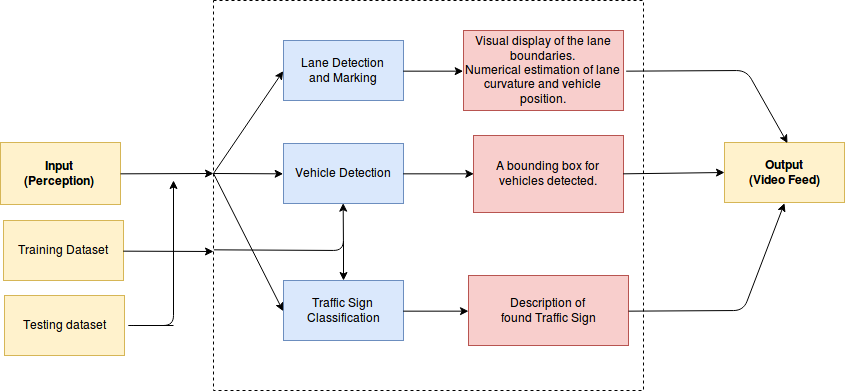
\includegraphics[scale=0.5]{Architecture.png}
\caption{Architecture Diagram}
\end{center}
\end{figure}
\begin{enumerate}
\item
Input: System will capture input using action camera as live video feed.
\item
Lane Detection and Marking module will split video into frames and will detect edges, lane boundaries.It will also produce numerical estimation of lane curvature and vehicle postion

\item
Vehicle Detection module will use classifier to classify objects in video frame as car or not car. It will produce cascade windows for objects classified as cars.


\item
Traffic sign classification module will use classifier to classify traffic signs in video frame. It will produce description of every sign.

\item
Output: Video feed with annotations from all the modules.


\end{enumerate}

\newpage
\noindent
\section{Probable deadline for Project completion}
Last week of March - 2018.

\section{References}
\begin{enumerate}
\item
Raman Maini \& Dr. Himanshu Aggarwal , “Study and Comparison of Various Image Edge Detection Techniques”, International Journal of Image Processing (IJIP), Volume (3) : Issue (1)
\item
Stallkamp, J, Schlipsing, M, Salmen, J, and Igel, C. The German Traffic Sign Recognition Benchmark: A multi-class classification competition. In International Joint Conference on Neural Networks, 2011.
\item 
Nguwi, Y.-Y and Kouzani, A. Detection and classification of road signs in natural environments. Neural Computing and Applications, 17:265–289, 2008. 10.1007/s00521-007-0120-z.

\end{enumerate}

\end{flushleft}
\end{document}

